\chapter{Introduction to Machine Learning and Neural Networks}
\label{chap:intro-ml-nn}

% Set section numbering depth
\setcounter{secnumdepth}{4}
\setcounter{tocdepth}{3}

\section{Introduction to Machine Learning}
\label{sec:intro-ml}

\subsection{What is Learning?}
\label{subsec:what-is-learning}

Learning is the process of acquiring new knowledge, skills, or behaviors through experience. This process transforms inputs—such as data, experiences, or information—into useful capabilities like expertise, new skills, or predictive models.

\subsubsection{Key Questions in Learning}
\label{subsubsec:key-questions-learning}

\begin{enumerate}
\item What are the essential inputs for the learning process?
\item How do we measure the effectiveness and success of learning?
\item What are the underlying mechanisms and processes by which learning occurs?
\end{enumerate}

\subsection{What is Reasoning?}
\label{subsec:what-is-reasoning}

Reasoning is the ability to draw logical conclusions from known facts or learned knowledge. Unlike learning, reasoning relies on logical inference rather than large amounts of data.

\subsection{From Animal Learning to Machine Learning}
\label{subsec:animal-to-ml}

\subsubsection{Example: Bait Shyness in Rats}
\label{subsubsec:bait-shyness-rats}

Rats demonstrate a fundamental learning principle through their feeding behavior:

\begin{enumerate}
\item They sample novel food cautiously
\item If the food causes illness, they avoid it in the future
\item Past experience directly informs future decisions
\end{enumerate}

This natural learning process parallels challenges in machine learning.

\subsubsection{Parallel: Spam Email Filtering}
\label{subsubsec:spam-filtering-parallel}

Consider how this biological learning principle applies to spam detection:

\begin{enumerate}
\item \textbf{Naive approach}: Memorize all past spam emails
\item \textbf{Problem}: Cannot classify previously unseen emails
\item \textbf{Solution}: Extract generalizable patterns (like words, phrases, or sender patterns)
\item \textbf{Key insight}: Both rats and spam filters must generalize from specific experiences to handle new, similar situations
\end{enumerate}

This ability to generalize leads us to examine the different types of reasoning that enable learning and decision-making.

\subsection{Types of Reasoning: Comprehensive Overview}
\label{subsec:types-reasoning}

\subsubsection{Inductive Reasoning}
\label{subsubsec:inductive-reasoning}

\textbf{Definition:} Inductive reasoning extracts patterns from observed data to make predictions about future or unseen cases. This approach moves from specific observations to general conclusions, yielding probable rather than certain results.

\textbf{Key Characteristics:}

\begin{enumerate}
\item Most prevalent form of reasoning in the animal kingdom and primary mode in machine learning
\item Forms the basis of most learned behaviors in animals  
\item Used extensively in deep learning and LLMs
\end{enumerate}

\paragraph{Examples Across Different Contexts}
\label{para:inductive-examples}

\textbf{Human Example}: Every cat I have ever seen has four legs. Therefore, all cats have four legs.

\textbf{Animal Example}:

\begin{itemize}
\item A dog learns that when its owner picks up the leash, it will probably go for a walk (experienced hundreds of times)
\item A squirrel learns that acorns are edible after eating many without getting sick
\end{itemize}

\textbf{Machine Learning Example}: A spam classifier learns from previously labeled emails and generalizes patterns to detect new spam messages

\textbf{LLM Example}: When asked to complete "The sky is blue because...", the model has "observed" this pattern countless times in training data and induces probable completions based on statistical patterns

\paragraph{Applications in AI/ML}
\label{para:inductive-applications}

\begin{enumerate}
\item Deep learning model training
\item Pattern recognition systems
\item Predictive analytics
\item Natural language processing
\end{enumerate}

\subsubsection{Deductive Reasoning}
\label{subsubsec:deductive-reasoning}

\textbf{Definition:} Deductive reasoning moves from general rules and premises to reach specific, guaranteed conclusions. It starts with a general rule and a specific case to reach a logical conclusion.

\textbf{Key Characteristics:}

\begin{enumerate}
\item Provides certainty when premises are true
\item Animals generally lack this capability for abstract reasoning
\item LLMs can only mimic this through pattern matching
\end{enumerate}

\paragraph{Examples Across Different Contexts}
\label{para:deductive-examples}

\textbf{Human Example}: All men are mortal. Socrates is a man. Therefore, Socrates is mortal.

\textbf{Mathematical Example}: If all squares have four sides and a shape is a square, it must have four sides.

\textbf{Animal Limitation}: Animals cannot perform abstract syllogistic reasoning, such as deducing that "because all felines are carnivores and a tiger is a feline, then a tiger is a carnivore."

\textbf{LLM Mimicry}: When given "All mammals have hair. A dolphin is a mammal. Therefore...", the model completes with "a dolphin has hair"—not through true logical syllogism, but by recognizing learned textual patterns from training data.

\paragraph{Applications in AI}
\label{para:deductive-applications}

\begin{enumerate}
\item Expert systems (traditional AI)
\item Symbolic reasoning systems
\item Theorem proving
\item Rule-based systems
\end{enumerate}

\paragraph{Limitations}
\label{para:deductive-limitations}

\begin{enumerate}
\item LLMs lack strict logical reasoning capabilities
\item Most modern AI systems don't use true deductive reasoning
\end{enumerate}

\subsubsection{Abductive Reasoning (Inference to Best Explanation)}
\label{subsubsec:abductive-reasoning}

\textbf{Definition:} Abductive reasoning starts with an observation and seeks to find the simplest and most likely explanation. It's the process of finding a hypothesis that, if true, would best explain the observation.

\paragraph{Key Characteristics}
\label{para:abductive-characteristics}

\begin{enumerate}
\item Often described as "inference to the best explanation"
\item Guesses the most probable explanation given incomplete data
\item Can be demonstrated in simple forms by animals
\item Simulated effectively by modern LLMs
\end{enumerate}

\paragraph{Examples Across Different Contexts}
\label{para:abductive-examples}

\textbf{Human Example}: The grass is wet. A plausible explanation is that it rained (most likely, though sprinklers are possible).

\textbf{Medical Example}: A doctor observes symptoms like fever and cough and infers the patient likely has the flu.

\textbf{Animal Example}:

\begin{itemize}
\item A squirrel hears rustling and sees movement, "abduces" it's a predator and climbs a tree
\item A raven sees a human place a rock over food, infers the food is under the rock when human leaves
\end{itemize}

\textbf{LLM Example}: When asked "Why is the road wet?", generates explanations like "It rained," "Water main broke," or "Street cleaner passed" by ranking probable explanations from training data.

\paragraph{Applications in AI/ML}
\label{para:abductive-applications}

\begin{enumerate}
\item Medical diagnosis systems
\item Troubleshooting AI
\item Natural language understanding
\item Creative writing and content generation
\end{enumerate}

\paragraph{In Machine Learning Systems}
\label{para:abductive-ml-systems}

\textbf{Hypothesis Generation}: ML models generate predictions based on learned patterns - they present the most probable explanation without "knowing" it's true.

\textbf{Bayesian Inference}: AI systems use Bayesian models to start with prior beliefs and update them as new evidence is presented.

\subsubsection{Analogical Reasoning (Pattern Transfer)}
\label{subsubsec:analogical-reasoning}

\textbf{Definition:} Analogical reasoning applies knowledge from one context to another by recognizing similar patterns or relationships.

\paragraph{Applications in AI/ML}
\label{para:analogical-applications}

\begin{enumerate}
\item AI-powered tutoring systems
\item Cross-domain learning
\item Transfer learning in neural networks
\end{enumerate}

\paragraph{Example}
\label{para:analogical-example}

AI that learns human speech patterns in English and transfers that learning to generate speech in another language.

\subsubsection{Bayesian Reasoning (Probabilistic Prediction)}
\label{subsubsec:bayesian-reasoning}

\textbf{Definition:} Bayesian reasoning uses probability to predict outcomes by updating beliefs based on new evidence.

\paragraph{Applications in AI/ML}
\label{para:bayesian-applications}

\begin{enumerate}
\item Spam filtering systems
\item AI language models
\item Uncertainty quantification
\end{enumerate}

\paragraph{Example}
\label{para:bayesian-example}

A Bayesian spam filter assigns probabilities to words appearing in spam emails and calculates the likelihood that a new email is spam.

\subsubsection{Causal Reasoning (Understanding Cause-and-Effect)}
\label{subsubsec:causal-reasoning}

\textbf{Definition:} Causal reasoning determines causal relationships rather than just correlations.

\paragraph{Limitations in Current AI}
\label{para:causal-limitations}

\begin{enumerate}
\item LLMs struggle with true causality
\item Most AI systems identify correlations rather than causes
\end{enumerate}

\paragraph{Example}
\label{para:causal-example}

In healthcare, researchers identify that smoking causes lung cancer, rather than just observing that smokers have higher cancer rates.

\subsubsection{Counterfactual Reasoning (What-If Thinking)}
\label{subsubsec:counterfactual-reasoning}

\textbf{Definition:} Counterfactual reasoning explores hypothetical scenarios and alternative possibilities.

\paragraph{Applications in AI}
\label{para:counterfactual-applications}

\begin{enumerate}
\item Risk analysis systems
\item AI decision-making
\item Simulation and planning
\end{enumerate}

\paragraph{Example}
\label{para:counterfactual-example}

A self-driving car AI simulates different driving scenarios to decide the safest course of action in an emergency.

\subsection{Reasoning Capabilities Across Intelligence Types}
\label{subsec:reasoning-capabilities}

\begin{table}[h!]
\centering
\begin{tabular}{|p{2.5cm}|p{3cm}|p{3.5cm}|p{3cm}|}
\hline
\textbf{Reasoning Type} & \textbf{Animals} & \textbf{Large Language Models} & \textbf{Traditional AI} \\
\hline
\textbf{Inductive} & Primary (survival-focused) & Primary (pattern-based) & Limited \\
\hline
\textbf{Deductive} & Absent (complex forms) & Simulated (pattern matching) & Primary (rule-based) \\
\hline
\textbf{Abductive} & Limited (simple forms) & Effective (learned patterns) & Limited \\
\hline
\textbf{Causal} & Basic & Limited & Rule-dependent \\
\hline
\textbf{Adaptability} & High (within domain) & High (pattern recognition) & Low (manual updates) \\
\hline
\end{tabular}
\caption{Reasoning Capabilities Across Intelligence Types}
\label{tab:reasoning-capabilities}
\end{table}

While inductive reasoning is powerful, it has inherent limitations that both animals and AI systems must navigate.

\subsection{Limitations of Inductive Reasoning}
\label{subsec:inductive-limitations}

\subsubsection{Pigeon Superstition Experiment (B.F. Skinner)}
\label{subsubsec:pigeon-superstition}

This experiment demonstrated how animals can form false associations through inductive reasoning.

\subsubsection{Garcia \& Koelling Experiment (1966)}
\label{subsubsec:garcia-koelling}

This landmark experiment studied \textbf{selective associative learning} in rats and demonstrated that \textbf{not all stimuli are equally associated} with consequences.

\paragraph{Experimental Design}
\label{para:garcia-design}

Researchers used a compound stimulus approach:

\begin{enumerate}
\item \textbf{Taste component}: Saccharin-flavored water
\item \textbf{Audiovisual component}: Lights and sounds during drinking
\end{enumerate}

Rats were then exposed to different aversive consequences:

\begin{enumerate}
\item \textbf{Group 1}: Illness (nausea from mild radiation or toxin)
\item \textbf{Group 2}: Physical discomfort (mild electric shocks)
\end{enumerate}

\paragraph{Results}
\label{para:garcia-results}

\textbf{Illness-Induced Group:}

\begin{enumerate}
\item Developed strong aversion to taste cues (saccharin water)
\item Showed minimal aversion to audiovisual cues
\end{enumerate}

\textbf{Shock-Induced Group:}

\begin{enumerate}
\item Developed strong aversion to audiovisual cues (lights and sounds)  
\item Showed no aversion to taste cues
\end{enumerate}

\textbf{Key Finding:} Rats selectively associated specific stimuli with appropriate consequences—taste with illness, external cues with physical danger.

\paragraph{Scientific Impact}
\label{para:garcia-impact}

This experiment revolutionized learning theory by:

\begin{enumerate}
\item \textbf{Challenging equipotentiality}: Not all stimulus-response associations are equally learnable
\item \textbf{Demonstrating biological constraints}: Evolution shapes what animals can easily learn
\item \textbf{Revealing adaptive biases}: Learning mechanisms evolved to enhance survival
\begin{enumerate}
\item Taste naturally links to internal consequences (poisoning)
\item External cues (sounds, lights) link to external threats (predators)
\end{enumerate}
\end{enumerate}

\paragraph{Implications for Machine Learning}
\label{para:garcia-implications}

\begin{enumerate}
\item \textbf{Learning requires inductive bias}: Not all associations are equally learnable
\item \textbf{Feature relevance varies}: Some inputs are more informative than others  
\item \textbf{Domain knowledge matters}: Evolutionary or expert-designed constraints improve learning
\item \textbf{No universal learner exists}: All learning algorithms must make assumptions (No-Free-Lunch theorem)
\end{enumerate}

These biological insights directly inform machine learning design, where inductive bias plays a crucial role in model performance.

\subsection{Inductive Bias in Machine Learning}
\label{subsec:inductive-bias-ml}

\subsubsection{What is Inductive Bias?}
\label{subsubsec:what-is-inductive-bias}

\textbf{Definition:} Inductive bias refers to the set of assumptions that a learning algorithm makes to generalize from limited training data to unseen data.

\textbf{Why is it Critical?}

Inductive bias is essential because:

\begin{enumerate}
\item Machine learning models have limited training data
\item Models must generalize from past observations to unseen cases  
\item Without appropriate bias, models may overfit (memorizing training data without learning generalizable patterns)
\end{enumerate}

\subsubsection{Types of Inductive Biases}
\label{subsubsec:types-inductive-bias}

\paragraph{Preference for Simpler Models (Occam's Razor)}
\label{para:occam-razor}

\begin{enumerate}
\item \textbf{Assumption}: Simpler explanations are preferred over complex ones
\item \textbf{Example}: Decision trees with fewer splits are preferred because they generalize better
\item \textbf{In Deep Learning}: Regularization techniques ($L_1$, $L_2$) penalize complex models
\end{enumerate}

\paragraph{Smoothness Assumption}
\label{para:smoothness-assumption}

\begin{enumerate}
\item \textbf{Assumption}: Data points that are close together should have similar outputs
\item \textbf{Example}: In image classification, two similar images should belong to the same class
\item \textbf{In ML}: K-Nearest Neighbors (KNN) assumes nearby data points have the same label
\end{enumerate}

\paragraph{Similar Features Should Have Similar Effects}
\label{para:similar-features}

\begin{enumerate}
\item \textbf{Assumption}: If two features are related, their effects should be similar
\item \textbf{Example}: In linear regression, correlated features often have similar coefficients
\end{enumerate}

\paragraph{Prior Knowledge About the Task (Domain-Specific Bias)}
\label{para:domain-specific-bias}

\begin{enumerate}
\item \textbf{Assumption}: Certain relationships are more likely in specific tasks
\item \textbf{Example}: In NLP, word order matters
\item \textbf{In ML}: Transformers use positional embeddings to capture sentence structure
\end{enumerate}

\paragraph{Invariance Bias (Translation, Rotation, Scale Invariance)}
\label{para:invariance-bias}

\begin{enumerate}
\item \textbf{Assumption}: Some transformations should not change predictions
\item \textbf{Example}: Rotating an image of a cat should still classify it as a cat
\item \textbf{In ML}: CNNs use convolutional filters to enforce translation invariance
\end{enumerate}

\paragraph{Sparsity Assumption}
\label{para:sparsity-assumption}

\begin{enumerate}
\item \textbf{Assumption}: Only a few features are truly important
\item \textbf{Example}: In text classification, most words are irrelevant
\item \textbf{In ML}: $L_1$ regularization forces models to select important features
\end{enumerate}

These general principles manifest differently across various neural network architectures, each designed with specific inductive biases for particular tasks.

\subsection{Inductive Bias in Specific Architectures}
\label{subsec:inductive-bias-architectures}

\subsubsection{Convolutional Neural Networks (CNNs)}
\label{subsubsec:cnn-inductive-bias}

CNNs are designed for image processing and rely on three key inductive biases:

\paragraph{Locality Bias (Local Connectivity)}
\label{para:locality-bias}

\begin{enumerate}
\item \textbf{Assumption}: Nearby pixels are more relevant than distant pixels
\item \textbf{Example}: In facial recognition, CNN detects eyes, nose, mouth before recognizing entire face
\end{enumerate}

\paragraph{Translation Invariance}
\label{para:translation-invariance}

\begin{enumerate}
\item \textbf{Assumption}: An object should be recognized regardless of position
\item \textbf{How it works}: CNNs use shared convolutional filters
\item \textbf{Example}: Handwritten digit "3" recognized anywhere in the image
\end{enumerate}

\paragraph{Hierarchical Feature Learning}
\label{para:hierarchical-features}

\begin{enumerate}
\item \textbf{Assumption}: Complex patterns learned by stacking abstraction layers
\item \textbf{Example}: Lower layers detect edges → middle layers detect shapes → deeper layers detect objects
\end{enumerate}

\subsubsection{Recurrent Neural Networks (RNNs \& LSTMs)}
\label{subsubsec:rnn-inductive-bias}

RNNs are designed for sequential data and rely on:

\paragraph{Temporal Dependency Bias}
\label{para:temporal-dependency}

\begin{enumerate}
\item \textbf{Assumption}: Recent information is more important than distant past
\item \textbf{Example}: In "The cat sat on the mat", nearby words are more related
\end{enumerate}

\paragraph{Order Sensitivity Bias}
\label{para:order-sensitivity}

\begin{enumerate}
\item \textbf{Assumption}: The order of input elements matters
\item \textbf{Example}: "Dog bites man" $\neq$ "Man bites dog"
\end{enumerate}

\subsubsection{Transformers (BERT, GPT)}
\label{subsubsec:transformer-inductive-bias}

\paragraph{Attention-Based Bias (Self-Attention)}
\label{para:attention-bias}

\begin{enumerate}
\item \textbf{Assumption}: Important words can be anywhere in a sentence
\item \textbf{Example}: In "The dog chased the ball...which was blue", "which" refers to "ball"
\end{enumerate}

\paragraph{Context-Aware Learning Bias}
\label{para:context-aware-bias}

\begin{enumerate}
\item \textbf{Assumption}: Word meaning depends on context
\item \textbf{Example}: "Bank" can mean financial institution or riverbank
\end{enumerate}

\paragraph{Positional Encoding Bias}
\label{para:positional-encoding}

\begin{enumerate}
\item \textbf{Assumption}: Order matters even without sequential processing
\item \textbf{Example}: "She ate an apple" $\neq$ "An apple ate she"
\end{enumerate}

\subsection{Machine Learning vs Other Approaches}
\label{subsec:ml-vs-other}

\subsubsection{Why Machine Learning?}
\label{subsubsec:why-ml}

\begin{enumerate}
\item For many problems, it's difficult to program correct behavior by hand
\item Examples: recognizing objects in images, understanding human speech
\item Machine learning approach: program an algorithm to automatically learn from data
\end{enumerate}

\subsubsection{Reasons to Use Learning Algorithms}
\label{subsubsec:reasons-learning-algorithms}

\begin{enumerate}
\item Hard to code up a solution by hand (e.g., vision, speech)
\item System needs to adapt to changing environment (e.g., spam detection)
\item Want system to perform better than human programmers
\item Privacy/fairness considerations (e.g., ranking search results)
\end{enumerate}

\subsubsection{Machine Learning vs Statistics}
\label{subsubsec:ml-vs-statistics}

\begin{table}[h!]
\centering
\begin{tabular}{|p{3cm}|p{5cm}|p{5cm}|}
\hline
\textbf{Aspect} & \textbf{Statistics} & \textbf{Machine Learning} \\
\hline
\textbf{Primary Goal} & Draw valid conclusions for scientists/policymakers & Build autonomous predictive systems \\
\hline
\textbf{Focus} & Interpretability and mathematical rigor & Predictive performance and scalability \\
\hline
\textbf{Approach} & Hypothesis testing and inference & Pattern recognition and automation \\
\hline
\end{tabular}
\caption{Machine Learning vs Statistics}
\label{tab:ml-vs-statistics}
\end{table}

\subsubsection{Relations to AI}
\label{subsubsec:relations-to-ai}

\begin{itemize}
\item AI does not always imply a learning-based system
\item \textbf{Non-learning AI approaches}:
\begin{enumerate}
\item Symbolic reasoning
\item Rule-based systems
\item Tree search
\end{enumerate}
\item \textbf{Learning-based systems}:
\begin{enumerate}
\item Learned based on data
\item More flexibility
\item Good at solving pattern recognition problems
\end{enumerate}
\end{itemize}

\subsection{Symbolic AI vs Machine Learning}
\label{subsec:symbolic-vs-ml}

\subsubsection{What is Symbolic AI?}
\label{subsubsec:what-is-symbolic-ai}

\begin{enumerate}
\item Also known as \textbf{Good Old-Fashioned AI (GOFAI)}
\item Represents knowledge using \textbf{symbols, rules, and logic}
\item Uses \textbf{explicitly programmed rules} for reasoning
\item Based on \textbf{formal logic, tree search, and knowledge representation}
\item \textbf{Example}: If "All humans are mortal" and "Socrates is human", then "Socrates is mortal"
\end{enumerate}

\subsubsection{Tree Search in Symbolic AI}
\label{subsubsec:tree-search-symbolic}

\begin{enumerate}
\item Fundamental approach for solving problems by exploring decision trees
\item Uses algorithms like DFS, BFS, and A* Search
\item \textbf{Example}: Chess AI searches possible future board states
\item Does \textbf{not generalize from data} but computes solutions using logical steps
\end{enumerate}

\subsubsection{Rule-Based AI}
\label{subsubsec:rule-based-ai}

\begin{itemize}
\item Subset of Symbolic AI using \textbf{explicit if-then rules}
\item Rules manually defined by experts
\item \textbf{Examples}:
\begin{enumerate}
\item IF patient has fever AND cough $\rightarrow$ Diagnose as flu
\item IF transaction > \$10,000 $\rightarrow$ Flag as potential fraud
\end{enumerate}
\item \textbf{Limitation}: Struggles with exceptions and uncertain scenarios
\end{itemize}

\subsubsection{Symbolic AI vs Machine Learning Comparison}
\label{subsubsec:symbolic-vs-ml-comparison}

\begin{table}[h!]
\centering
\begin{tabular}{|p{3cm}|p{4.5cm}|p{4.5cm}|}
\hline
\textbf{Feature} & \textbf{Symbolic AI} & \textbf{Machine Learning} \\
\hline
\textbf{Knowledge Source} & Rules \& logic & Data \& patterns \\
\hline
\textbf{Interpretability} & Highly explainable & Often a black box \\
\hline
\textbf{Adaptability} & Rigid (manual updates) & Can generalize from data \\
\hline
\textbf{Data Requirements} & Minimal & Requires large datasets \\
\hline
\textbf{Best Use Cases} & Theorem proving, expert systems & NLP, computer vision, recommendations \\
\hline
\end{tabular}
\caption{Symbolic AI vs Machine Learning Comparison}
\label{tab:symbolic-vs-ml}
\end{table}

\subsubsection{Limitations of Symbolic AI}
\label{subsubsec:symbolic-limitations}

\begin{enumerate}
\item Difficult to scale—requires manual updates
\item Cannot handle unstructured data (images, speech)
\item Struggles with uncertainty—rules don't adapt
\item Machine Learning outperforms in perception tasks
\end{enumerate}

\subsubsection{The Future: Hybrid AI (Neuro-Symbolic AI)}
\label{subsubsec:hybrid-ai}

\begin{enumerate}
\item Combines \textbf{Symbolic AI (structured logic)} with \textbf{Machine Learning (pattern recognition)}
\item \textbf{Example}: AI lawyer uses Symbolic AI for legal rules + ML for case history analysis
\item Enhances \textbf{explainability, adaptability, and reasoning}
\end{enumerate}

\subsection{Role of Prior Knowledge}
\label{subsec:prior-knowledge}

The effectiveness of any learning system—biological or artificial—depends heavily on the prior knowledge and assumptions it brings to new situations.

\textbf{Key Principles:}

\begin{enumerate}
\item \textbf{Prior knowledge accelerates learning}: Domain expertise makes learning from examples more efficient
\item \textbf{Trade-offs exist}: Stronger assumptions improve performance on expected tasks but reduce flexibility for unexpected scenarios  
\item \textbf{Balance is crucial}: The optimal learning system finds the right equilibrium between prior knowledge and data-driven adaptation
\item \textbf{Tool development matters}: Creating methods to incorporate domain expertise remains central to advancing machine learning theory
\end{enumerate}

\subsection{Key Takeaways}
\label{subsec:key-takeaways-ml}

\subsubsection{Fundamental Principles}
\label{subsubsec:fundamental-principles-ml}

\begin{enumerate}
\item \textbf{Learning transforms experience into generalizable knowledge} through pattern recognition and abstraction
\item \textbf{Inductive bias is essential} for effective learning—all successful learning systems require appropriate assumptions about their domain
\item \textbf{No universal learner exists}—every learning algorithm must make trade-offs based on its intended use case
\end{enumerate}

\subsubsection{Reasoning in AI Systems}
\label{subsubsec:reasoning-ai-systems}

\begin{enumerate}
\item \textbf{Biological systems} primarily use inductive reasoning, with limited abductive capabilities
\item \textbf{Traditional AI systems} excel at deductive reasoning but struggle with adaptation
\item \textbf{Modern ML/LLMs} are powerful at inductive reasoning and can simulate other reasoning types through pattern matching
\item \textbf{Future AI systems} will likely combine symbolic reasoning with machine learning for enhanced interpretability and robust decision-making
\end{enumerate}

\subsubsection{Practical Implications}
\label{subsubsec:practical-implications}

\begin{enumerate}
\item \textbf{Domain knowledge matters}—incorporating appropriate inductive biases improves learning efficiency and generalization
\item \textbf{Architecture design is crucial}—different neural network architectures embed specific assumptions about data structure (CNNs for images, Transformers for sequences)
\item \textbf{Learning and reasoning are complementary}—effective AI systems need both the ability to learn from data and to reason with acquired knowledge
\end{enumerate}

\section{Neural Networks: From Computation to Biology}
\label{sec:nn-computation-biology}

\subsection{What is Computation?}
\label{subsec:what-is-computation}

\textbf{Computation} is the process of performing calculations, manipulating data, or executing a sequence of operations to solve problems or transform inputs into desired outputs. It encompasses both the theoretical and practical aspects of processing information.

\subsubsection{Core Elements of Computation}
\label{subsubsec:core-elements-computation}

Every computational process involves these fundamental components:

\begin{enumerate}
\item \textbf{Input}: Data or information that enters the system
\item \textbf{Processing}: The manipulation or transformation of that data according to specific rules or algorithms
\item \textbf{Output}: The result or solution produced by the processing
\item \textbf{Algorithm}: The step-by-step procedure or set of rules that defines how the processing should occur
\item \textbf{Storage/Memory}: The ability to retain information for use during or after processing
\end{enumerate}

\subsubsection{Types of Computation}
\label{subsubsec:types-computation}

\paragraph{Mathematical Computation}
\label{para:mathematical-computation}

\begin{enumerate}
\item Numerical calculations (arithmetic, calculus, statistics)
\item Symbolic manipulation (algebra, logic)
\item Optimization problems
\end{enumerate}

\paragraph{Logical Computation}
\label{para:logical-computation}

\begin{enumerate}
\item Boolean operations (AND, OR, NOT)
\item Decision-making processes
\item Pattern matching and recognition
\end{enumerate}

\paragraph{Data Processing}
\label{para:data-processing}

\begin{enumerate}
\item Sorting and searching
\item Data transformation and analysis
\item Information retrieval
\end{enumerate}

\paragraph{Algorithmic Computation}
\label{para:algorithmic-computation}

\begin{enumerate}
\item Following predefined procedures
\item Recursive processes
\item Iterative methods
\end{enumerate}

\subsection{Computational Models: Theoretical Foundations}
\label{subsec:computational-models}

A \textbf{computational model} is a mathematical or conceptual framework that defines how computation is carried out. It provides the rules and structure for describing:

\begin{enumerate}
\item \textbf{What can be computed}
\item \textbf{How it can be computed}
\item \textbf{The limits of computation}
\end{enumerate}

\subsubsection{Elements Common to All Computational Models}
\label{subsubsec:elements-computational-models}

\begin{enumerate}
\item \textbf{Representation of Information (Data Model)}\\
   Defines how information is stored (symbols, numbers, states, molecules, etc.)

\item \textbf{Operators / Rules}\\
   Defines how information is transformed (functions, state transitions, reactions, etc.)

\item \textbf{Control Mechanism}\\
   Defines the order of operations (sequential steps, parallel updates, probabilistic choices)

\item \textbf{Storage / Memory}\\
   Defines how intermediate information is kept and reused (tape, registers, neuron activations)

\item \textbf{Input / Output}\\
   Defines how external data enters and results leave the system
\end{enumerate}

\subsubsection{Elementary Components of Any Computing Model}
\label{subsubsec:elementary-components}

What are the elementary components of any conceivable computing model? In the theory of general recursive functions, for example, it is possible to reduce any computable function to some composition rules and a small set of primitive functions. For a universal computer, we ask about the existence of a minimal and sufficient instruction set.

For an arbitrary computing model, the following metaphoric expression has been proposed:

\begin{equation}
\label{eq:computation-formula}
\textbf{computation} = \textbf{storage} + \textbf{transmission} + \textbf{processing}
\end{equation}

The mechanical computation of a function presupposes that these three elements are present:

\begin{enumerate}
\item \textbf{Storage}: Data can be stored and maintained over time
\item \textbf{Transmission}: Information can be communicated to the functional units of the model  
\item \textbf{Processing}: Data can be transformed according to computational rules
\end{enumerate}

It is implicitly assumed that a certain \textbf{coding} of the data has been agreed upon. Coding plays an important role in information processing because, as Claude Shannon showed in 1948, when noise is present information can still be transmitted without loss, if the right code with the right amount of redundancy is chosen.

\paragraph{How Different Models Implement These Components}
\label{para:model-implementations}

\textbf{Modern Computers:}

\begin{enumerate}
\item Transform storage of information into a form of information transmission
\item Static memory chips store a bit as a circulating current until the bit is read
\item Separation between storage (RAM/disk) and processing (CPU) with data buses for transmission
\end{enumerate}

\textbf{Turing Machines:}

\begin{enumerate}
\item Store information on an infinite tape
\item Transmission is performed by the read-write head moving along the tape
\item Processing occurs through state transitions based on current symbol and state
\end{enumerate}

\textbf{Cellular Automata:}

\begin{enumerate}
\item Store information in each cell
\item Each cell acts simultaneously as storage and a small processor
\item Transmission occurs through local neighborhood interactions between adjacent cells
\item No separation between storage, transmission, and processing - they are unified in each cell
\end{enumerate}

\subsection{Four Fundamental Computational Models}
\label{subsec:four-computational-models}

\subsubsection{Turing Machine (Alan Turing, 1936)}
\label{subsubsec:turing-machine}

\textbf{The Foundation of Algorithmic Computation}

\begin{itemize}
\item \textbf{Style:} Imperative / mechanical model of computation
\item \textbf{Core Idea:} A machine reads/writes symbols on an infinite tape with a finite set of rules
\item \textbf{Representation:}
\begin{enumerate}
\item Infinite tape divided into cells
\item Head that can read/write and move left or right
\item Finite state machine controlling transitions
\end{enumerate}
\item \textbf{Strengths:}
\begin{enumerate}
\item Canonical model for algorithmic computability
\item Basis of the Church–Turing Thesis
\item Directly models sequential execution
\end{enumerate}
\item \textbf{Limitations:}
\begin{enumerate}
\item Low-level, not efficient
\item Sequential by nature, doesn't capture parallelism well
\end{enumerate}
\end{itemize}

\textbf{Example:} A Turing Machine can simulate any algorithm you'd run on a modern computer (given enough tape).

\subsubsection{Lambda Calculus (Alonzo Church, 1930s)}
\label{subsubsec:lambda-calculus}

\textbf{The Foundation of Functional Computation}

\begin{itemize}
\item \textbf{Style:} Functional model of computation
\item \textbf{Core Idea:} Everything is a function. Computation = function application + substitution
\item \textbf{Representation:}
\begin{enumerate}
\item Variables ($x$)
\item Function definitions ($\lambda x. \text{expression}$)
\item Function application ($(f \; x)$)
\end{enumerate}
\item \textbf{Strengths:}
\begin{enumerate}
\item Basis of functional programming (Haskell, Lisp)
\item Good for reasoning about higher-order functions, abstraction, recursion
\end{enumerate}
\item \textbf{Limitations:}
\begin{enumerate}
\item Abstract and symbolic; not naturally tied to hardware
\item Efficiency is not modeled, just computability
\end{enumerate}
\end{itemize}

\textbf{Example:} Addition can be defined entirely in terms of functions (Church numerals).

\subsubsection{Cellular Automata (Stanislaw Ulam, John von Neumann, later Conway)}
\label{subsubsec:cellular-automata}

\textbf{The Foundation of Distributed/Parallel Computation}

\begin{itemize}
\item \textbf{Style:} Spatial / distributed model of computation
\item \textbf{Core Idea:} Computation arises from simple local rules applied to a grid of cells over time
\item \textbf{Representation:}
\begin{enumerate}
\item Infinite (or finite) grid of cells
\item Each cell has a finite state (e.g., alive/dead)
\item Transition rules depend only on the local neighborhood
\end{enumerate}
\item \textbf{Strengths:}
\begin{enumerate}
\item Good for modeling parallel, distributed, physical systems
\item Supports universal computation (Conway's Life is Turing-complete)
\end{enumerate}
\item \textbf{Limitations:}
\begin{enumerate}
\item Not natural for symbolic or algebraic computation
\item More suited for simulating dynamics
\end{enumerate}
\end{itemize}

\textbf{Example:} Conway's \textit{Game of Life} shows how simple rules produce complex, even universal, behaviors.

\subsubsection{Biological Computation (Inspired by Nature)}
\label{subsubsec:biological-computation}

\textbf{The Foundation of Adaptive/Learning Computation}

Biological models are inspired by living systems and emphasize parallelism, adaptability, and learning.

\textbf{Key Characteristics:}

\begin{enumerate}
\item \textbf{Learns from data} (training) rather than using fixed rules
\item Massive parallelism and fault tolerance
\item Self-organization and adaptation
\item Pattern recognition and generalization
\end{enumerate}

\subsection{Modern Computing Systems: From Theory to Practice}
\label{subsec:modern-computing-systems}

\subsubsection{Central Processing Unit (CPU) - \textit{Based on Turing Machine Model}}
\label{subsubsec:cpu-turing-model}

\begin{enumerate}
\item \textbf{Representation:} Binary data in registers and memory
\item \textbf{Operators:} Instruction set (add, move, compare, jump)
\item \textbf{Control:} Program counter + clock cycle (sequential execution)
\item \textbf{Storage:} Cache, RAM, hard disk
\item \textbf{Input/Output:} Peripherals, buses, I/O ports
\end{enumerate}

\subsubsection{Graphics Processing Unit (GPU) - \textit{Based on Cellular Automata Model}}
\label{subsubsec:gpu-cellular-model}

\begin{enumerate}
\item \textbf{Representation:} Data stored in many cores and VRAM
\item \textbf{Operators:} SIMD (single-instruction, multiple-data) kernels running in parallel
\item \textbf{Control:} Thousands of threads execute simultaneously under scheduling
\item \textbf{Storage:} VRAM, shared memory on cores
\item \textbf{Input/Output:} Typically streams of data for graphics or AI workloads
\end{enumerate}

\subsubsection{Neural Network Systems - \textit{Based on Biological Computation Model}}
\label{subsubsec:nn-biological-model}

\begin{enumerate}
\item \textbf{Representation:} Weights and activations (usually floating-point numbers)
\item \textbf{Operators:} Linear algebra (matrix multiply, convolution, activation functions)
\item \textbf{Control:} Layer-by-layer propagation (forward/backward pass)
\item \textbf{Storage:} Model parameters + learned weights
\item \textbf{Input/Output:} Input features (image, text) $\rightarrow$ Output predictions
\end{enumerate}

\subsection{Biological Neural Networks: Nature's Computational Model}
\label{subsec:biological-neural-networks}

\subsubsection{Characteristics of Biological Neural Networks}
\label{subsubsec:characteristics-biological-nn}

The following are key characteristics that make biological neural networks powerful computational systems:

\begin{enumerate}
\item \textbf{(a) Highly interconnected:} Neurons form a complex web of connections
\item \textbf{(b) Robustness and Fault Tolerance:} The decay of nerve cells does not affect the overall function of the network significantly
\item \textbf{(c) Flexibility:} The ability to reorganize and adapt to new situations
\item \textbf{(d) Handling incomplete information:} Ability to infer appropriate outputs even when some inputs are missing or noisy
\item \textbf{(e) Parallel processing:} Multiple neurons can process information simultaneously
\end{enumerate}

\subsubsection{Neuron Structure}
\label{subsubsec:neuron-structure}

\begin{figure}[h!]
\centering
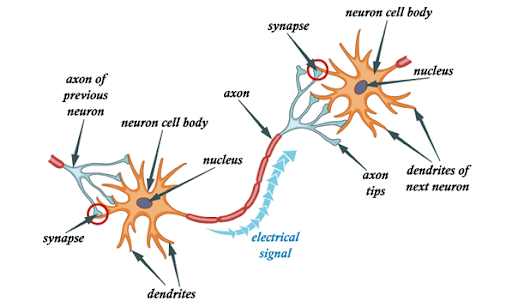
\includegraphics[width=0.8\textwidth]{figures/biological_neuron.png}
\caption{Structure of a biological neuron}
\label{fig:biological-neuron}
\end{figure}

\paragraph{Components of a Neuron}
\label{para:neuron-components}

\begin{enumerate}
\item \textbf{Fundamental unit:} neuron (cell body / soma, dendrites, axon, synapses)
\item \textbf{Dendrites} receive inputs; \textbf{axon} transmits output and branches to many synapses (often thousands)
\item \textbf{Synapse:} junction between axon terminal and target cell
\item \textbf{Synaptic junctions} form between presynaptic axon terminals and postsynaptic dendrites or the cell body
\item \textbf{Typical sizes:}
\begin{itemize}
\item soma $\sim$ 10–80 $\mu$m
\item synaptic gap $\sim$ 200 nm
\item neuron length from 0.01 mm to 1 m
\end{itemize}
\end{enumerate}

\subsubsection{Signal Transmission and Firing}
\label{subsubsec:signal-transmission}

\begin{enumerate}
\item \textbf{Resting potential} $\sim$ -70 mV; depolarization above threshold (roughly $\sim$10 mV) triggers firing
\item \textbf{Action potentials} are all-or-none pulses sent down the axon; information is encoded in firing rate ($\sim$1–100 Hz)
\item \textbf{Propagation speed} in brain tissue $\sim$ 0.5–2 m/s; synaptic transmission delay $\sim$ 0.5 ms
\item After firing the membrane recovers (\textbf{refractory period}); synaptic effects decay with time constant $\sim$5–10 ms
\end{enumerate}

\subsubsection{Synapses: Chemistry and Types}
\label{subsubsec:synapses}

\begin{enumerate}
\item \textbf{Transmission} across synapse is chemical: neurotransmitters released from presynaptic terminal
\item \textbf{Postsynaptic effect} can be excitatory (depolarizing) or inhibitory (hyperpolarizing)
\item All endings of a given axon are typically either excitatory or inhibitory
\item \textbf{Synaptic strength} depends on activity and can change over time (basis for learning)
\end{enumerate}

\subsubsection{Plasticity and Learning}
\label{subsubsec:plasticity-learning}

\begin{enumerate}
\item Active synapses that repeatedly contribute to postsynaptic firing tend to strengthen; inactive ones weaken
\item \textbf{Hebb's rule} ("cells that fire together, wire together") describes this activity-dependent plasticity
\item Continuous modification of synaptic strengths underlies learning and memory formation
\end{enumerate}

\subsubsection{Network-Scale Properties}
\label{subsubsec:network-scale-properties}

\begin{enumerate}
\item \textbf{Convergence/divergence:} neurons receive many inputs and send outputs to many others
\item \textbf{Average inputs per neuron:} on the order of $10^4$ synapses; total synaptic connections in human brain estimated $\sim 10^{15}$
\item The cortex contains extremely dense, layered networks with vast numbers of interconnected neurons
\item Studying simple, identical units helps understand complex brain functions, but full understanding remains far off
\end{enumerate}

\subsubsection{Cortical Layers: Input/Output Organization}
\label{subsubsec:cortical-layers}

The cerebral cortex is organized into six distinct layers, each with specialized roles in processing and routing information. This laminar organization is crucial for understanding how biological neural networks process information hierarchically.

\paragraph{Cortical Layers \& Their Input/Output Functions}
\label{para:cortical-layers-functions}

\begin{figure}[h!]
\centering
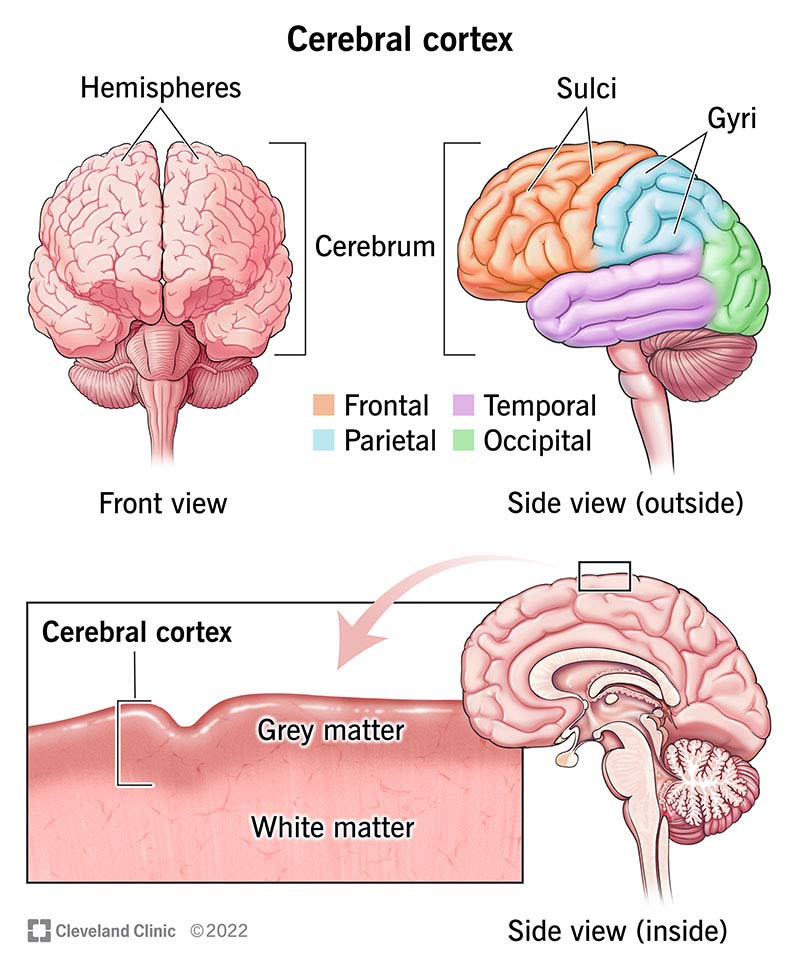
\includegraphics[width=0.6\textwidth]{/latex/figures/cerebral_cortex.png}
\caption{Cortical layers organization}
\label{fig:cortical-layers}
\end{figure}

\begin{table}[h!]
\centering
\scriptsize
\begin{tabular}{|p{0.8cm}|p{2.5cm}|p{3cm}|p{3cm}|p{3.5cm}|}
\hline
\textbf{Layer} & \textbf{Name (Common)} & \textbf{Main Cell Types / Features} & \textbf{Input Roles} & \textbf{Output / Projection Roles} \\
\hline
\textbf{I} & Molecular (Plexiform) layer & Few neurons; apical dendritic tufts of pyramidal neurons; horizontal fibers; Cajal-Retzius cells; glial cells & Receives feedback / modulatory inputs; integrates signal from other cortical areas; contributes to modulation of how input is processed & Minimal direct long-range output; mainly modulatory interactions \\
\hline
\textbf{II} & External Granular layer & Stellate (granular) cells + small pyramidal cells & Inputs from other cortical areas; association fibers & Outputs to adjacent cortical columns; corticocortical communication \\
\hline
\textbf{III} & External Pyramidal layer & Pyramidal cells of small-to-medium size; many horizontal/corticocortical fibers & Receives input from other cortex; association inputs & Sends outputs to other parts of cortex; communicates between cortical areas \\
\hline
\textbf{IV} & Internal Granular (Lamina IV) & Stellate cells mainly; some pyramidal cells; receiving thalamic inputs & Major input hub: thalamic sensory afferents predominantly arrive here & Sends processed signals upwards to layers II \& III and across column \\
\hline
\textbf{V} & Internal Pyramidal layer & Large pyramidal cells; size/shape suited to long projection & Receives processed cortical input & Major output layer to subcortical targets (e.g., brainstem, spinal cord), other cortical areas \\
\hline
\textbf{VI} & Multiform / Fusiform layer & Mixed cell types: fusiform, pyramidal, interneurons; connects deeper to thalamus & Receives inputs from other cortical layers \& some feedback loops & Sends feedback to thalamus; helps modulate incoming signals; also outputs to other cortical/subcortical regions \\
\hline
\end{tabular}
\caption{Cortical Layers and Their Functions}
\label{tab:cortical-layers}
\end{table}

\paragraph{Functional Specialization by Cortical Area}
\label{para:functional-specialization}

\textbf{Sensory Processing Areas} (e.g., visual cortex):

\begin{enumerate}
\item Have a very prominent Layer IV (strong input) because they process raw sensory data
\item Dense thalamic inputs require robust input processing capabilities
\end{enumerate}

\textbf{Motor Areas}:

\begin{enumerate}
\item Layer V is very prominent (strong output) since these regions send commands out to body/motor systems
\item Large pyramidal neurons in Layer V can project long distances to motor targets
\end{enumerate}

\textbf{Association Areas}:

\begin{enumerate}
\item Rely heavily on Layers II \& III for inter-cortical communication and integration
\item Process and integrate information from multiple sensory and cognitive sources
\end{enumerate}

\textbf{Thalamic Feedback}:

\begin{enumerate}
\item Layer VI helps regulate what inputs are emphasized (gain control, feedback)
\item Provides top-down modulation of sensory processing
\end{enumerate}

\paragraph{Example Information Flow in Cortical Processing}
\label{para:information-flow-cortical}

\begin{enumerate}
\item \textbf{Sensory Input}: Sensory afferents from thalamus $\rightarrow$ hit Layer IV in primary sensory cortex
\item \textbf{Vertical Processing}: Signals go up $\rightarrow$ processed and passed through Layers II \& III to adjacent/association cortical areas
\item \textbf{Integration \& Decision}: Higher-level processing / decision made $\rightarrow$ Layers V / VI send back outputs (motor commands, feedback to thalamus)
\item \textbf{Modulation}: Modulatory feedback (Layer I and VI) helps adjust sensitivity, attention, integration
\end{enumerate}

This layered organization demonstrates how biological neural networks implement hierarchical processing, with clear separation of input processing, integration, output generation, and modulatory control - principles that have influenced the design of artificial neural network architectures.

\subsection{Other Biological Computation Models}
\label{subsec:other-biological-models}

\subsubsection{DNA Computing}
\label{subsubsec:dna-computing}

\begin{enumerate}
\item Uses DNA strands and biochemical reactions to encode and solve problems
\item Enables \textbf{massive parallelism} (billions of molecules interacting at once)
\item Example: Adleman (1994) solved a small Hamiltonian Path problem with DNA
\end{enumerate}

\subsubsection{Membrane Computing (P Systems)}
\label{subsubsec:membrane-computing}

\begin{enumerate}
\item Inspired by biological cells with membranes
\item Computation modeled as molecules passing between compartments with rules
\end{enumerate}

\subsubsection{Immune System Computation}
\label{subsubsec:immune-system-computation}

\begin{enumerate}
\item Inspired by adaptive immune systems recognizing pathogens
\item Used in anomaly detection, cybersecurity, adaptive algorithms
\end{enumerate}

\subsubsection{Swarm Intelligence}
\label{subsubsec:swarm-intelligence}

\begin{enumerate}
\item Inspired by ants, bees, and bird flocks
\item Simple agents interacting lead to complex global solutions
\item Example: Ant Colony Optimization for shortest path problems
\end{enumerate}

\subsection{Comparative Analysis of Computational Models}
\label{subsec:comparative-analysis}

\subsubsection{Key Differences Between Models}
\label{subsubsec:key-differences-models}

\begin{table}[h!]
\centering
\scriptsize
\begin{tabular}{|p{2cm}|p{2.5cm}|p{2.5cm}|p{2.5cm}|p{3cm}|}
\hline
\textbf{Feature} & \textbf{Lambda Calculus} & \textbf{Cellular Automata} & \textbf{Turing Machine} & \textbf{Biological Computation} \\
\hline
\textbf{Paradigm} & Functional & Distributed / Parallel & Imperative / Sequential & Adaptive / Parallel / Learning \\
\hline
\textbf{Representation} & Functions + substitution & Grid of cells + local rules & Tape + head + state machine & Neurons, DNA, agents, molecules \\
\hline
\textbf{Best for} & Reasoning about functions \& programs & Modeling physical systems & Defining algorithms \& computability & Learning, adaptation, biological processes \\
\hline
\textbf{Computational Power} & Universal (Turing-complete) & Universal (e.g., Game of Life) & Universal (baseline model) & Universal (many models are Turing-complete) \\
\hline
\textbf{Origin} & Church (1930s) & Ulam, von Neumann, Conway (1940s–70s) & Turing (1936) & 1990s onward (Adleman, Hopfield, etc.) \\
\hline
\end{tabular}
\caption{Key Differences Between Computational Models}
\label{tab:computational-models-comparison}
\end{table}

\subsubsection{Mapping to Modern Computing Technologies}
\label{subsubsec:mapping-modern-tech}

\paragraph{Lambda Calculus $\rightarrow$ Functional Programming Languages}
\label{para:lambda-to-functional}

\begin{enumerate}
\item \textbf{Influence:} Functional languages like Haskell, Lisp, OCaml, Scala
\item \textbf{Practice:} Used in compilers, parallelism, AI/ML frameworks (TensorFlow graphs)
\item \textbf{Example:} Python's \texttt{lambda} functions (\texttt{map(lambda x: x*2, list)})
\end{enumerate}

\paragraph{Cellular Automata $\rightarrow$ Parallel / Distributed Computing}
\label{para:cellular-to-parallel}

\begin{enumerate}
\item \textbf{Influence:} Inspiration for GPU architectures, parallel algorithms, simulations
\item \textbf{Practice:} Physics simulations, cryptography, GPU computations
\item \textbf{Example:} Conway's Game of Life on GPUs
\end{enumerate}

\paragraph{Turing Machine $\rightarrow$ CPUs \& Algorithms}
\label{para:turing-to-cpu}

\begin{enumerate}
\item \textbf{Influence:} CPUs $\approx$ optimized Turing machines (memory = tape, registers = head)
\item \textbf{Practice:} Von Neumann architecture, algorithm design, compilers
\item \textbf{Example:} Any code on a CPU is compiled down to Turing-like steps
\end{enumerate}

\paragraph{Biological Computation $\rightarrow$ AI and Unconventional Computing}
\label{para:biological-to-ai}

\begin{enumerate}
\item \textbf{Influence:} Inspired deep learning, DNA-based computation, swarm optimization
\item \textbf{Practice:} Neural networks in AI, bioinformatics, optimization, cybersecurity
\item \textbf{Example:} Deep learning models (vision, NLP), DNA algorithms, ant colony optimization
\end{enumerate}

\subsubsection{Modern Technology Mapping Overview}
\label{subsubsec:modern-tech-mapping}

\begin{table}[h!]
\centering
\begin{tabular}{|p{3cm}|p{4cm}|p{5cm}|}
\hline
\textbf{Model} & \textbf{Modern Counterpart} & \textbf{Where It Shows Up} \\
\hline
Lambda Calculus & Functional languages, ML frameworks & Haskell, Lisp, TensorFlow, PyTorch \\
\hline
Cellular Automata & GPUs, Parallel computing, Simulation & Physics engines, cryptography \\
\hline
Turing Machine & CPUs, von Neumann architecture, Algorithms & Everyday programming, OS, compilers \\
\hline
Biological Computation & Neural networks, DNA computing, swarm intelligence & AI, optimization, bioinformatics \\
\hline
\end{tabular}
\caption{Modern Technology Mapping}
\label{tab:modern-tech-mapping}
\end{table}

\subsection{Key Insights and Takeaways}
\label{subsec:key-insights-computation}

\subsubsection{From Biological Neural Networks}
\label{subsubsec:insights-biological-nn}

\begin{enumerate}
\item Neurons are simple units whose structure (dendrite/axon/synapse) enables complex computation
\item Signals are electrical within neurons and chemical at synapses; timing and rate carry information
\item Synaptic plasticity provides a biological basis for learning (Hebbian adaptation)
\item Massive connectivity (many synapses per neuron, $\sim 10^{15}$ total) creates powerful, distributed processing
\end{enumerate}

\subsubsection{From Computational Models}
\label{subsubsec:insights-computational-models}

\begin{enumerate}
\item \textbf{Lambda Calculus:} Computation = function evaluation
\item \textbf{Turing Machine:} Computation = manipulating symbols step by step
\item \textbf{Cellular Automata:} Computation = local rule interactions on grids
\item \textbf{Biological Computation:} Computation = adaptive processes inspired by nature
\end{enumerate}

\subsubsection{Universal Principles}
\label{subsubsec:universal-principles}

All four computational models are \textbf{Turing-complete}, meaning they can solve the same class of problems, but they represent different metaphors for thinking about computation:

\begin{enumerate}
\item \textbf{Sequential vs. Parallel:} Some models naturally express parallel computation (cellular automata, biological systems) while others are inherently sequential (Turing machines)

\item \textbf{Static vs. Adaptive:} Traditional models use fixed rules, while biological models can learn and adapt their behavior

\item \textbf{Abstract vs. Physical:} Some models are mathematical abstractions (lambda calculus) while others are inspired by physical or biological processes

\item \textbf{Efficiency vs. Universality:} All models can theoretically solve the same problems, but they differ greatly in practical efficiency for different types of tasks
\end{enumerate}

\subsection{The Journey from Computation to Intelligence}
\label{subsec:journey-computation-intelligence}

This document traces the path from fundamental computational concepts to sophisticated biological neural networks:

\begin{enumerate}
\item \textbf{Computation} provides the basic framework for information processing
\item \textbf{Computational Models} offer different paradigms for organizing computation
\item \textbf{Modern Computing Systems} implement these models in physical hardware
\item \textbf{Biological Systems} demonstrate how computation can emerge naturally and adapt
\item \textbf{Artificial Neural Networks} attempt to capture the power of biological computation in engineered systems
\end{enumerate}

Understanding this progression helps us appreciate both the theoretical foundations of computation and the remarkable achievements of biological evolution in creating intelligent systems. It also provides insight into why artificial neural networks, inspired by biology but implemented on digital computers, have become such powerful tools for machine learning and artificial intelligence.

\subsection{Artificial Neural Networks}
\label{subsec:artificial-neural-networks}

\subsubsection{Introduction: From Biology to Computation}
\label{subsubsec:biology-to-computation}

Artificial Neural Networks (ANNs) represent one of the most successful attempts to harness the computational principles observed in biological neural systems for solving complex problems. Unlike traditional algorithmic approaches that follow explicit step-by-step instructions, neural networks learn to solve problems through experience and pattern recognition, much like biological brains.

\subsubsection{Fundamental Architecture: Primitive Functions and Composition Rules}
\label{subsubsec:fundamental-architecture}

To understand artificial neural networks, we must first examine their core computational elements. Every computational model requires:

\begin{enumerate}
\item \textbf{Primitive Functions}: Basic operations that cannot be decomposed further
\item \textbf{Composition Rules}: Ways to combine primitive functions to create complex behaviors
\end{enumerate}

\paragraph{Primitive Functions in Neural Networks}
\label{para:primitive-functions-nn}

In artificial neural networks, \textbf{primitive functions are located in the nodes (neurons) of the network}. Each node implements a specific mathematical transformation that processes incoming information and produces an output.

\paragraph{Composition Rules in Neural Networks}
\label{para:composition-rules-nn}

The \textbf{composition rules are contained implicitly in}:

\begin{enumerate}
\item \textbf{Interconnection pattern of the nodes}: How neurons are connected determines information flow
\item \textbf{Synchrony or asynchrony of information transmission}: Whether neurons update simultaneously or in sequence
\item \textbf{Presence or absence of cycles}: Whether information can flow in loops (recurrent networks) or only forward (feedforward networks)
\end{enumerate}

This differs fundamentally from traditional computing models:

\begin{table}[h!]
\centering
\begin{tabular}{|p{4cm}|p{4cm}|p{4cm}|}
\hline
\textbf{Computing Model} & \textbf{Primitive Functions} & \textbf{Composition Rules} \\
\hline
\textbf{von Neumann Processor} & Machine instructions (ADD, MOVE, JUMP) & Program sequence + control flow \\
\hline
\textbf{Artificial Neural Networks} & Neuron activation functions & Network topology + connection weights + timing \\
\hline
\end{tabular}
\caption{Computing Models Comparison}
\label{tab:computing-models-comparison}
\end{table}

\subsubsection{The Abstract Neuron: Building Block of Intelligence}
\label{subsubsec:abstract-neuron}

\paragraph{Structure of an Abstract Neuron}
\label{para:structure-abstract-neuron}

An abstract neuron with $n$ inputs processes information through the following components:

\paragraph{Abstract Neuron Architecture}
\label{para:abstract-neuron-architecture}

\begin{figure}[h!]
\centering
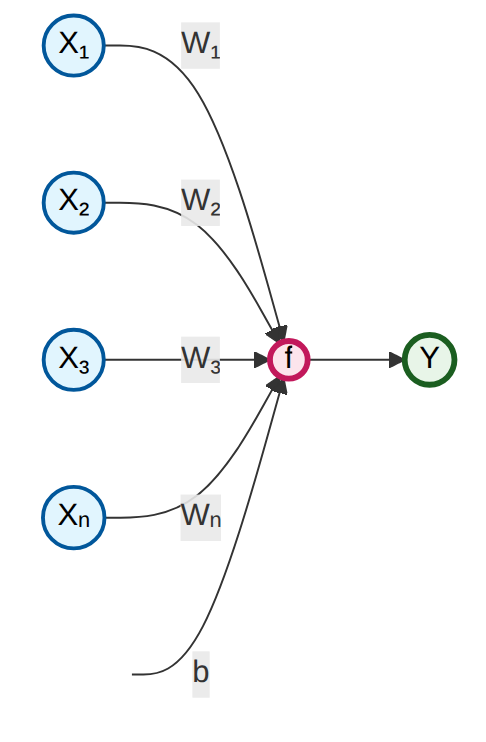
\includegraphics[width=0.8\textwidth]{diagrams/abstract_neuron.png}
\caption{Abstract Neuron Architecture}
\label{fig:abstract-neuron}
\end{figure}

\begin{equation}
\label{eq:neuron-output}
Y = f\left(w_1 x_1 + w_2 x_2 + \cdots + w_n x_n\right)
\end{equation}

\textbf{Key Components:}

\begin{enumerate}
\item \textbf{Input Channels}: Each input channel $i$ can transmit a real value $X_i$
\item \textbf{Weights}: Each input has an associated weight $W_i$ that multiplies the incoming information
\item \textbf{Integration}: The weighted signals are combined (usually by summation)
\item \textbf{Primitive Function}: An activation function $f$ transforms the integrated signal
\item \textbf{Output}: The result is transmitted to connected neurons
\end{enumerate}

\paragraph{Mathematical Representation}
\label{para:mathematical-representation-neuron}

The output of a neuron can be expressed as:

\begin{equation}
\label{eq:neuron-general}
Y = f\left(\sum_{i=1}^{n} W_i X_i + b\right)
\end{equation}

Where:

\begin{itemize}
\item $Y$: Output of the neuron
\item $f$: Activation function (primitive function)
\item $W_i$: Weight associated with input $i$
\item $X_i$: Value of input $i$
\item $b$: Bias term (optional constant)
\end{itemize}

\subsubsection{Neural Networks as Function Approximators}
\label{subsubsec:nn-function-approximators}

\paragraph{Networks of Primitive Functions}
\label{para:networks-primitive-functions}

\textbf{Artificial neural networks are nothing but networks of primitive functions.} Each node transforms its input into a precisely defined output, and the combination of these transformations creates complex computational behaviors.

\paragraph{The Network Function}
\label{para:network-function}

Consider a neural network that takes inputs $(x, y, z)$ and produces an output through nodes implementing primitive functions $f_1, f_2, f_3, f_4$. The network can be thought of as implementing a \textbf{network function $\phi$}:

\begin{equation}
\label{eq:network-function}
\phi(x, y, z) = f_4\left(a_4 \cdot f_3\left(a_3 \cdot f_2\left(a_2 \cdot f_1(a_1 \cdot x)\right)\right) + \ldots\right)
\end{equation}

Where $a_1, a_2, \ldots, a_5$ are the weights of the network. \textbf{Different selections of weights produce different network functions.}

\paragraph{Three Critical Elements}
\label{para:three-critical-elements}

Different models of artificial neural networks differ mainly in three fundamental aspects:

\begin{enumerate}
\item \textbf{Structure of the Nodes}
\begin{itemize}
\item Choice of activation function (sigmoid, ReLU, tanh, etc.)
\item Input integration method (weighted sum, product, etc.)
\item Presence of bias terms
\end{itemize}

\item \textbf{Topology of the Network}
\begin{itemize}
\item Feedforward vs. recurrent connections
\item Number of layers and neurons per layer
\item Connection patterns (fully connected, sparse, convolutional)
\end{itemize}

\item \textbf{Learning Algorithm}
\begin{itemize}
\item Method for finding optimal weights
\item Supervised vs. unsupervised vs. reinforcement learning
\item Optimization techniques (gradient descent, evolutionary algorithms)
\end{itemize}
\end{enumerate}

\subsubsection{Function Approximation: The Classical Problem}
\label{subsubsec:function-approximation-classical}

\paragraph{Historical Context}
\label{para:historical-context-function-approx}

Function approximation is a classical problem in mathematics: \textbf{How can we reproduce a given function $F : \mathbb{R} \to \mathbb{R}$ either exactly or approximately using a given set of primitive functions?}

Traditional approaches include:

\begin{enumerate}
\item \textbf{Polynomial approximation}: Using powers of $x$ (Taylor series)
\item \textbf{Fourier approximation}: Using trigonometric functions (sine and cosine)
\item \textbf{Spline approximation}: Using piecewise polynomials
\end{enumerate}

\paragraph{Neural Networks as Universal Approximators}
\label{para:nn-universal-approximators}

Neural networks provide a revolutionary approach to function approximation:

\textbf{Key Insight}: With sufficient neurons and appropriate activation functions, neural networks can approximate any continuous function to arbitrary precision (Universal Approximation Theorem).

\paragraph{Advantages of Neural Network Approximation}
\label{para:advantages-nn-approximation}

\begin{enumerate}
\item \textbf{Adaptive}: Networks learn the approximation from data rather than requiring explicit mathematical formulation
\item \textbf{Flexible}: Can handle high-dimensional inputs and complex, non-linear relationships
\item \textbf{Robust}: Can generalize to unseen data and handle noise
\item \textbf{Parallel}: Multiple neurons can process different aspects of the input simultaneously
\end{enumerate}

\subsubsection{Comparison: Classical vs. Neural Approximation}
\label{subsubsec:classical-vs-neural}

\paragraph{Taylor Series Neural Networks}
\label{para:taylor-series-nn}

As demonstrated in our earlier diagrams, neural networks can explicitly implement classical approximation methods:

\textbf{Taylor Series}: $F(x) = a_0 + a_1(x - x_0) + a_2(x - x_0)^2 + \ldots + a_n(x - x_0)^n$

\begin{enumerate}
\item \textbf{Basis Functions}: Powers of $(x - x_0)$
\item \textbf{Coefficients}: Learned as weights in the network
\item \textbf{Best For}: Local approximation around expansion point $x_0$
\end{enumerate}

\paragraph{Fourier Series Neural Networks}
\label{para:fourier-series-nn}

\textbf{Fourier Series}: $F(x) = \sum_{i=0}^{\infty} \left[a_i \cos(ix) + b_i \sin(ix)\right] = \sum_{i=0}^{\infty} w_i \sin(k_i x + d_i)$

\begin{enumerate}
\item \textbf{Basis Functions}: Trigonometric functions (sine/cosine)
\item \textbf{Coefficients}: Learned as weights and phase factors
\item \textbf{Best For}: Periodic functions and signal processing
\end{enumerate}

\paragraph{General Neural Networks}
\label{para:general-nn}

\textbf{Modern ANNs}: $F(x) = f_n\left(W_n \cdot f_{n-1}\left(W_{n-1} \cdot \ldots f_1(W_1 \cdot x + b_1) + b_{n-1}\right) + b_n\right)$

\begin{enumerate}
\item \textbf{Basis Functions}: Learned automatically through hidden layers
\item \textbf{Coefficients}: All weights and biases learned from data
\item \textbf{Best For}: Complex, high-dimensional problems without known mathematical structure
\end{enumerate}

\subsubsection{Learning in Neural Networks}
\label{subsubsec:learning-nn}

\paragraph{The Learning Problem}
\label{para:learning-problem}

Given:

\begin{itemize}
\item A set of input-output pairs: $\{(x_1, y_1), (x_2, y_2), \ldots, (x_m, y_m)\}$
\item A network architecture
\end{itemize}

\textbf{Goal}: Find weights $W$ and biases $b$ such that the network function $\phi(x; W, b)$ approximates the target function as closely as possible.

\paragraph{Learning as Optimization}
\label{para:learning-optimization}

\textbf{Objective}: Minimize the error between network outputs and desired outputs:

\begin{equation}
\label{eq:learning-objective}
E(W, b) = \sum_{i=1}^{m} \|\phi(x_i; W, b) - y_i\|^2
\end{equation}

\textbf{Method}: Use gradient-based optimization (backpropagation) to iteratively adjust weights:

\begin{align}
\label{eq:weight-update}
W &\leftarrow W - \eta \nabla_W E(W, b) \\
b &\leftarrow b - \eta \nabla_b E(W, b)
\end{align}

Where $\eta$ is the learning rate.

\subsubsection{Types of Neural Network Architectures}
\label{subsubsec:types-nn-architectures}

\paragraph{Feedforward Networks}
\label{para:feedforward-networks}

\begin{enumerate}
\item Information flows in one direction from input to output
\item No cycles or loops
\item Examples: Perceptrons, Multi-layer Perceptrons (MLPs)
\end{enumerate}

\paragraph{Recurrent Networks}
\label{para:recurrent-networks}

\begin{enumerate}
\item Contain cycles that allow information to persist
\item Can process sequences and exhibit temporal dynamics
\item Examples: RNNs, LSTMs, GRUs
\end{enumerate}

\paragraph{Convolutional Networks}
\label{para:convolutional-networks}

\begin{enumerate}
\item Specialized for processing grid-like data (images)
\item Use shared weights and local connectivity
\item Examples: CNNs, ResNets, Vision Transformers
\end{enumerate}

\paragraph{Specialized Architectures}
\label{para:specialized-architectures}

\begin{enumerate}
\item \textbf{Autoencoders}: Learn compressed representations
\item \textbf{GANs}: Generate new data similar to training examples
\item \textbf{Transformers}: Process sequences with attention mechanisms
\end{enumerate}

\subsubsection{Modern Applications and Impact}
\label{subsubsec:modern-applications}

\paragraph{Computer Vision}
\label{para:computer-vision-applications}

\begin{enumerate}
\item \textbf{Image Classification}: Recognizing objects in photographs
\item \textbf{Object Detection}: Finding and localizing objects
\item \textbf{Image Generation}: Creating realistic synthetic images
\end{enumerate}

\paragraph{Natural Language Processing}
\label{para:nlp-applications}

\begin{enumerate}
\item \textbf{Machine Translation}: Converting text between languages
\item \textbf{Language Models}: Understanding and generating human language
\item \textbf{Sentiment Analysis}: Determining emotional tone of text
\end{enumerate}

\paragraph{Scientific Computing}
\label{para:scientific-computing-applications}

\begin{enumerate}
\item \textbf{Physics Simulations}: Solving partial differential equations
\item \textbf{Drug Discovery}: Predicting molecular properties
\item \textbf{Climate Modeling}: Understanding complex environmental systems
\end{enumerate}

\subsubsection{Key Insights and Future Directions}
\label{subsubsec:key-insights-future}

\paragraph{Fundamental Principles}
\label{para:fundamental-principles-nn}

\begin{enumerate}
\item \textbf{Distributed Representation}: Information is stored across many neurons rather than in specific locations
\item \textbf{Emergent Computation}: Complex behaviors arise from simple neuron interactions
\item \textbf{Adaptive Learning}: Networks modify themselves based on experience
\item \textbf{Fault Tolerance}: Performance degrades gracefully with neuron damage
\end{enumerate}

\paragraph{Current Challenges}
\label{para:current-challenges-nn}

\begin{enumerate}
\item \textbf{Interpretability}: Understanding how networks make decisions
\item \textbf{Data Efficiency}: Learning from fewer examples
\item \textbf{Robustness}: Handling adversarial inputs and distribution shifts
\item \textbf{Energy Efficiency}: Reducing computational requirements
\end{enumerate}

\paragraph{Future Prospects}
\label{para:future-prospects-nn}

\begin{enumerate}
\item \textbf{Neuromorphic Computing}: Hardware that mimics brain architecture
\item \textbf{Quantum Neural Networks}: Leveraging quantum mechanics for computation
\item \textbf{Biological-Artificial Hybrids}: Integrating living neurons with artificial systems
\item \textbf{Continual Learning}: Networks that learn continuously without forgetting
\end{enumerate}

\subsubsection{Conclusion: The Power of Artificial Neural Networks}
\label{subsubsec:conclusion-ann-power}

Artificial neural networks represent a paradigm shift in computation - from explicit algorithmic programming to learning from data. By abstracting the key principles of biological neural computation (weighted connections, nonlinear transformations, and adaptive learning), ANNs have become one of the most powerful tools for solving complex problems in science, engineering, and everyday life.

The journey from understanding individual neurons to building networks capable of human-level performance in specific domains illustrates the power of \textbf{composition} - how simple primitive functions, when properly connected and trained, can give rise to remarkable computational abilities.

As we continue to develop more sophisticated architectures and learning algorithms, artificial neural networks promise to play an increasingly central role in our technological future, potentially leading us toward artificial general intelligence and beyond.

\begin{figure}[h!]
\centering
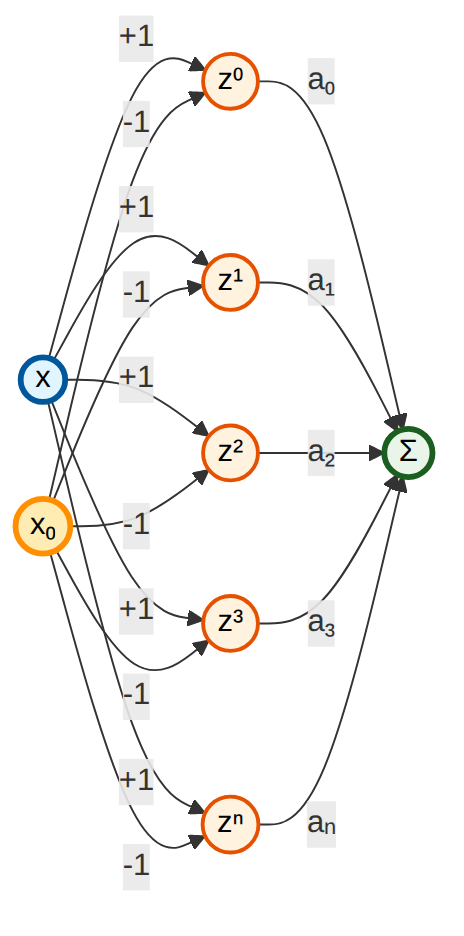
\includegraphics[width=0.8\textwidth]{diagrams/taylor_series_network.png}
\caption{Taylor Series Neural Network: $F(x) = a_0 + a_1(x - x_0) + a_2(x - x_0)^2 + \ldots + a_n(x - x_0)^n$}
\label{fig:taylor-series-network}
\end{figure}

\textbf{Network Architecture:}

\begin{enumerate}
\item \textbf{Input Layer}: Two inputs - $x$ (variable) and $x_0$ (expansion point/bias term)
\item \textbf{Polynomial Computation Layer}: Calculate basis functions $z^0, z^1, z^2, z^3, \ldots, z^n$
\begin{itemize}
\item $z^0 = (x-x_0)^0 = 1$ (constant term)
\item $z^1 = (x-x_0)^1$ (linear term)
\item $z^2 = (x-x_0)^2$ (quadratic term)
\item $z^3 = (x-x_0)^3$ (cubic term)
\item $z^n = (x-x_0)^n$ (nth-order term)
\end{itemize}
\item \textbf{Coefficient Neurons}: Learn the Taylor series coefficients $a_0, a_1, a_2, \ldots, a_n$
\item \textbf{Output}: Sum all weighted terms to approximate $F(x)$
\end{enumerate}

\textbf{Mathematical Mapping:}

\begin{enumerate}
\item \textbf{$a_0$ neuron}: Learns the constant coefficient $\times z^0$ (bias term)
\item \textbf{$a_1$ neuron}: Learns the linear coefficient $\times z^1$
\item \textbf{$a_2$ neuron}: Learns the quadratic coefficient $\times z^2$
\item \textbf{$a_3$ neuron}: Learns the cubic coefficient $\times z^3$
\item \textbf{$a_n$ neuron}: Learns the nth-order coefficient $\times z^n$
\end{enumerate}

\textbf{Key Features:}

\begin{enumerate}
\item \textbf{Dual Input Design}: $x$ and $x_0$ as separate inputs allows the network to learn both the function value and the optimal expansion point
\item \textbf{Explicit Basis Functions}: $z^0, z^1, z^2, \ldots, z^n$ clearly show the polynomial basis being computed
\item \textbf{Learnable Expansion Point}: $x_0$ can be treated as a learnable parameter (bias) or fixed reference point
\item \textbf{Modular Structure}: Each polynomial degree has its own computation and coefficient pathway
\end{enumerate}

This demonstrates how neural networks can implement \textbf{universal function approximation} by learning to combine polynomial basis functions, directly representing the mathematical foundation of Taylor series expansion through a structured network architecture.

\subsubsection{Fourier Series Neural Network}
\label{subsubsec:fourier-series-nn}

\begin{equation}
\label{eq:fourier-series}
F(x) = \sum_{i=0}^{\infty} a_i \cos(ix) + b_i \sin(ix) = \sum_{i=0}^{\infty} w_i \sin(k_i x + d_i)
\end{equation}

\begin{figure}[h!]
\centering
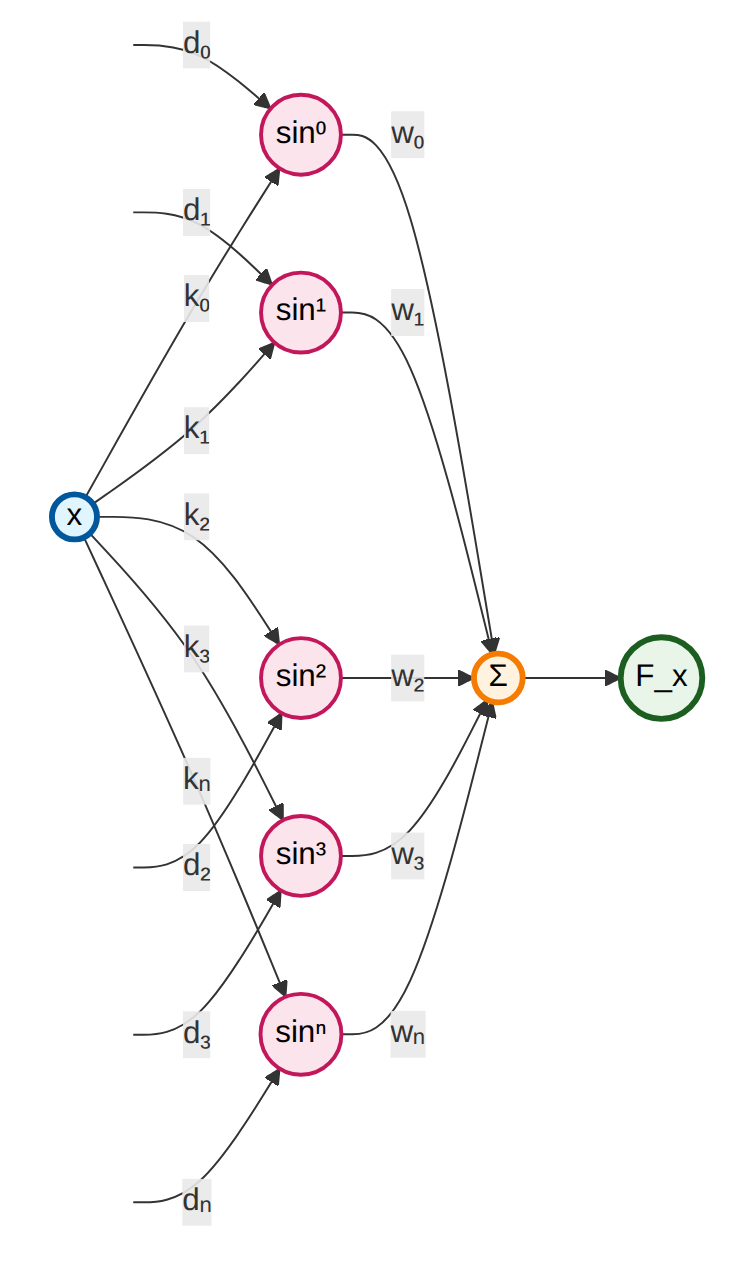
\includegraphics[width=0.8\textwidth]{diagrams/fourier_series_network.png}
\caption{Fourier Series Neural Network}
\label{fig:fourier-series-network}
\end{figure}

\textbf{Fourier Series Neural Network}: $F(x) = \sum_{i=0}^{\infty} \left[a_i \cos(ix) + b_i \sin(ix)\right]$

\textbf{Network Architecture:}

\begin{enumerate}
\item \textbf{Input Layer}: Single input $x$ (the variable)
\item \textbf{Trigonometric Basis Layer}: Calculate basis functions
\begin{itemize}
\item \textbf{Cosine terms}: $\cos^0(x) = 1$, $\cos^1(x) = \cos(x)$, $\cos^2(x) = \cos(2x)$, $\ldots$, $\cos^n(x) = \cos(nx)$
\item \textbf{Sine terms}: $\sin^1(x) = \sin(x)$, $\sin^2(x) = \sin(2x)$, $\sin^3(x) = \sin(3x)$, $\ldots$, $\sin^n(x) = \sin(nx)$
\end{itemize}
\item \textbf{Coefficient Neurons}: Learn the Fourier series coefficients
\begin{itemize}
\item \textbf{a-coefficients}: $a_0, a_1, a_2, a_3, \ldots, a_n$ for cosine terms
\item \textbf{b-coefficients}: $b_1, b_2, b_3, \ldots, b_n$ for sine terms
\end{itemize}
\item \textbf{Output}: Sum all weighted trigonometric terms to approximate $F(x)$
\end{enumerate}

\textbf{Mathematical Mapping:}

\begin{enumerate}
\item \textbf{$a_0$ neuron}: Learns the DC component (constant term) $\times \cos^0(x) = 1$
\item \textbf{$a_i$ neurons}: Learn cosine coefficients $\times \cos(ix)$ for harmonic frequencies
\item \textbf{$b_i$ neurons}: Learn sine coefficients $\times \sin(ix)$ for harmonic frequencies
\end{enumerate}

\textbf{Key Features:}

\begin{enumerate}
\item \textbf{Frequency Domain Representation}: Each neuron pair represents a specific harmonic frequency
\item \textbf{Orthogonal Basis Functions}: Sine and cosine functions form an orthogonal basis for periodic signals
\item \textbf{Harmonic Analysis}: Network learns to decompose signals into fundamental and harmonic components
\item \textbf{Periodic Function Approximation}: Particularly effective for modeling periodic and oscillatory phenomena
\end{enumerate}

\textbf{Comparison with Taylor Series:}

\begin{enumerate}
\item \textbf{Taylor}: Local polynomial approximation using powers of $(x-x_0)$
\item \textbf{Fourier}: Global trigonometric approximation using sine/cosine harmonics
\item \textbf{Taylor}: Best for smooth functions around expansion point
\item \textbf{Fourier}: Best for periodic functions and signal processing applications
\end{enumerate}

Both architectures demonstrate how neural networks can implement classical mathematical series expansions, providing structured approaches to \textbf{universal function approximation} through learned basis function combinations.

\subsubsection{Learning from Data: The Key Difference}
\label{subsubsec:learning-from-data}

The main difference between Taylor or Fourier series and artificial neural networks is, however, that \textbf{the function $F$ to be approximated is given not explicitly but implicitly through a set of input-output examples.} We know $F$ only at some points but we want to generalize as well as possible. This means that we try to adjust the parameters of the network in an optimal manner to reflect the information known and to extrapolate to new input patterns which will be shown to the network afterwards. This is the task of the learning algorithm used to adjust the network's parameters.

\paragraph{Classical Series vs. Neural Networks: A Fundamental Distinction}
\label{para:classical-vs-nn-distinction}

\textbf{Classical Mathematical Series (Taylor/Fourier):}

\begin{enumerate}
\item \textbf{Explicit Function Definition}: The function $F(x)$ is mathematically defined and known
\item \textbf{Analytical Coefficients}: Series coefficients can be computed directly using calculus
\begin{itemize}
\item Taylor: $a_n = \frac{F^{(n)}(x_0)}{n!}$ (nth derivative at expansion point)
\item Fourier: $a_n, b_n$ computed via integration over the function's period
\end{itemize}
\item \textbf{Perfect Representation}: Given enough terms, the series can represent the function exactly
\item \textbf{No Learning Required}: Coefficients are determined mathematically, not learned
\end{enumerate}

\textbf{Artificial Neural Networks:}

\begin{enumerate}
\item \textbf{Implicit Function Definition}: The function $F$ is unknown but represented by data points
\item \textbf{Learned Parameters}: Network weights and biases are learned from examples
\item \textbf{Approximation from Samples}: Must generalize from finite training data to unknown inputs
\item \textbf{Adaptive Learning}: Parameters adjust through iterative optimization algorithms
\end{enumerate}

\paragraph{The Learning Process: From Examples to Generalization}
\label{para:learning-process-generalization}

\textbf{Given:}

\begin{itemize}
\item Training dataset: $\{(x_1, F(x_1)), (x_2, F(x_2)), \ldots, (x_m, F(x_m))\}$
\item Neural network architecture with parameters $\theta$ (weights and biases)
\end{itemize}

\textbf{Goal:}
Find optimal parameters $\theta^*$ such that the network can:

\begin{enumerate}
\item \textbf{Fit the training data}: Network output $\approx F(x_i)$ for known examples
\item \textbf{Generalize to new inputs}: Network output $\approx F(x)$ for unseen $x$ values
\end{enumerate}

\textbf{Learning Algorithm Steps:}

\begin{enumerate}
\item \textbf{Initialize}: Set random initial values for all network parameters
\item \textbf{Forward Pass}: Compute network output for training examples
\item \textbf{Error Calculation}: Measure difference between network output and target values
\item \textbf{Backward Pass}: Compute gradients of error with respect to parameters
\item \textbf{Parameter Update}: Adjust parameters to reduce error
\item \textbf{Iteration}: Repeat until convergence or satisfactory performance
\end{enumerate}

\paragraph{Generalization: The Ultimate Test}
\label{para:generalization-ultimate-test}

The true power of neural networks lies in their ability to \textbf{extrapolate to new input patterns}:

\textbf{Training Phase:}

\begin{enumerate}
\item Network learns from limited examples
\item Parameters adjusted to minimize training error
\item Network discovers underlying patterns in the data
\end{enumerate}

\textbf{Testing Phase:}

\begin{enumerate}
\item Network encounters completely new inputs
\item Must produce reasonable outputs based on learned patterns
\item Success measured by generalization performance
\end{enumerate}

\textbf{Key Challenges:}

\begin{enumerate}
\item \textbf{Overfitting}: Learning training data too specifically, poor generalization
\item \textbf{Underfitting}: Insufficient learning capacity, poor performance on both training and test data
\item \textbf{Bias-Variance Tradeoff}: Balancing model complexity with generalization ability
\end{enumerate}

\subsubsection{Caveat: Biological Realism vs. Mathematical Abstraction}
\label{subsubsec:biological-realism-vs-abstraction}

In the theory of artificial neural networks we do not consider the whole complexity of real biological neurons. We only abstract some general principles and content ourselves with different levels of detail when simulating neural ensembles. The general approach is to conceive each neuron as a primitive function producing numerical results at some points in time. However, we can also think of artificial neurons as computing units which produce pulse trains in the way that biological neurons do. We can then simulate this behavior and look at the output of simple networks. This kind of approach, although more closely related to the biological paradigm, is still a very rough approximation of the biological processes.

\paragraph{Levels of Biological Abstraction}
\label{para:levels-biological-abstraction}

\textbf{Level 1: Mathematical Abstraction (Most Common)}

\begin{enumerate}
\item \textbf{Neuron Model}: Simple mathematical function $f\left(\sum w_i x_i + b\right)$
\item \textbf{Activation}: Continuous values (real numbers) representing firing rates
\item \textbf{Computation}: Matrix operations and gradient-based learning
\item \textbf{Advantages}: Computationally efficient, mathematically tractable
\item \textbf{Disadvantages}: Far removed from biological reality
\end{enumerate}

\textbf{Level 2: Rate-Based Models}

\begin{enumerate}
\item \textbf{Neuron Model}: Firing rate as a function of input
\item \textbf{Activation}: Continuous values representing average firing frequency
\item \textbf{Computation}: Differential equations modeling neural dynamics
\item \textbf{Advantages}: Captures some temporal dynamics
\item \textbf{Disadvantages}: Ignores individual spike timing
\end{enumerate}

\textbf{Level 3: Spiking Neural Networks}

\begin{enumerate}
\item \textbf{Neuron Model}: Explicit spike generation and propagation
\item \textbf{Activation}: Discrete spikes (pulse trains) with precise timing
\item \textbf{Computation}: Event-driven simulation of individual spikes
\item \textbf{Advantages}: More biologically realistic, captures temporal coding
\item \textbf{Disadvantages}: Computationally expensive, harder to train
\end{enumerate}

\textbf{Level 4: Detailed Biophysical Models}

\begin{enumerate}
\item \textbf{Neuron Model}: Multi-compartment models with ion channels
\item \textbf{Activation}: Detailed membrane potential dynamics
\item \textbf{Computation}: Partial differential equations for each neuron compartment
\item \textbf{Advantages}: High biological fidelity
\item \textbf{Disadvantages}: Extremely computationally intensive, limited scalability
\end{enumerate}

\paragraph{The Abstraction Trade-off}
\label{para:abstraction-tradeoff}

\textbf{Why We Abstract:}

\begin{enumerate}
\item \textbf{Computational Feasibility}: Detailed biological models are too complex for large networks
\item \textbf{Mathematical Tractability}: Simple models allow theoretical analysis and efficient learning algorithms
\item \textbf{Practical Performance}: Highly abstracted models often perform better on artificial tasks
\item \textbf{Understanding}: Simple models help us understand fundamental principles
\end{enumerate}

\textbf{What We Lose:}

\begin{enumerate}
\item \textbf{Temporal Dynamics}: Real neurons have complex temporal behavior and memory
\item \textbf{Spike Timing}: Information may be encoded in precise timing of spikes
\item \textbf{Metabolic Constraints}: Real neurons have energy limitations affecting computation
\item \textbf{Plasticity Mechanisms}: Biological learning is far more complex than gradient descent
\item \textbf{Network Topology}: Real brain networks have complex, evolved architectures
\end{enumerate}

\paragraph{Current Research Directions}
\label{para:current-research-directions}

\textbf{Bridging the Gap:}

\begin{enumerate}
\item \textbf{Neuromorphic Computing}: Hardware that mimics brain architecture and dynamics
\item \textbf{Spiking Neural Networks}: Incorporating temporal dynamics while maintaining trainability
\item \textbf{Biologically Plausible Learning}: Developing learning rules that could work in real brains
\item \textbf{Brain-Inspired Architectures}: Using insights from neuroscience to design better artificial networks
\end{enumerate}

\textbf{The Ongoing Challenge:}
Finding the right level of biological realism that maintains:

\begin{enumerate}
\item \textbf{Computational efficiency} for practical applications
\item \textbf{Theoretical understanding} of fundamental principles
\item \textbf{Biological inspiration} for novel architectures and algorithms
\item \textbf{Performance advantages} over purely mathematical approaches
\end{enumerate}

\paragraph{Implications for Understanding}
\label{para:implications-understanding}

This abstraction means that while artificial neural networks are \textbf{inspired by} biological systems, they should not be considered \textbf{models of} biological systems. They represent a successful engineering approach that captures some essential computational principles while sacrificing biological realism for practical performance.

\textbf{Key Takeaway}: Artificial neural networks are best understood as powerful mathematical tools for pattern recognition and function approximation, rather than as accurate simulations of brain function. Their success demonstrates that some principles of neural computation can be abstracted and applied effectively, even when divorced from their biological context.